\chapter{Grundlagen} \label{chap:grundlagen}

Das zweite Kapitel geht detailliert auf Convolutional Neural Networks (CNNs) ein. Es erklärt zunächst, wie \emph{Deep Neural Networks} (Oberkategorie von CNNs) aufgebaut sind bzw. trainiert werden können. Danach wird dargestellt, welche Durchbrüche speziell den Anlass zu CNNs gegeben haben, wie sich die Struktur von DNNs und CNNs voneinander unterscheiden und schließlich wie CNN-Schichten aus funktionaler Sicht aussehen.

\section{Deep Neural Network}

\subsection{Aufbau}

Die zu entwickelnden Algorithmen (Modelle) im datengetriebenen Ansatz in \autoref{sec:objectdetection} fallen unter die Kategorie Deep Neural Networks (auch \emph{Deep-Learning-Algorithmen} genannt). In der Regel besteht ein Deep Neural Network (DNN) aus einer \emph{Eingabeschicht}, einer \emph{Ausgabeschicht} und mindestens zwei \emph{verborgenen Schichten}. Jede Schicht setzt sich aus \emph{Neuronen} zusammen, die Informationen von anderen Neuronen oder von außen aufnehmen, modifizieren und als Ergebnis ausgeben. Jedes Neuron ist mit anderen Neuronen in der vorherigen sowie nächsten Schicht verbunden (siehe \autoref{fig:DNN}). Jede Verbindung bekommt bei der Initialisierung des Netzwerks ein zufälliges Anfangsgewicht zugeteilt.

\begin{figure}[!hb]
	\centering
	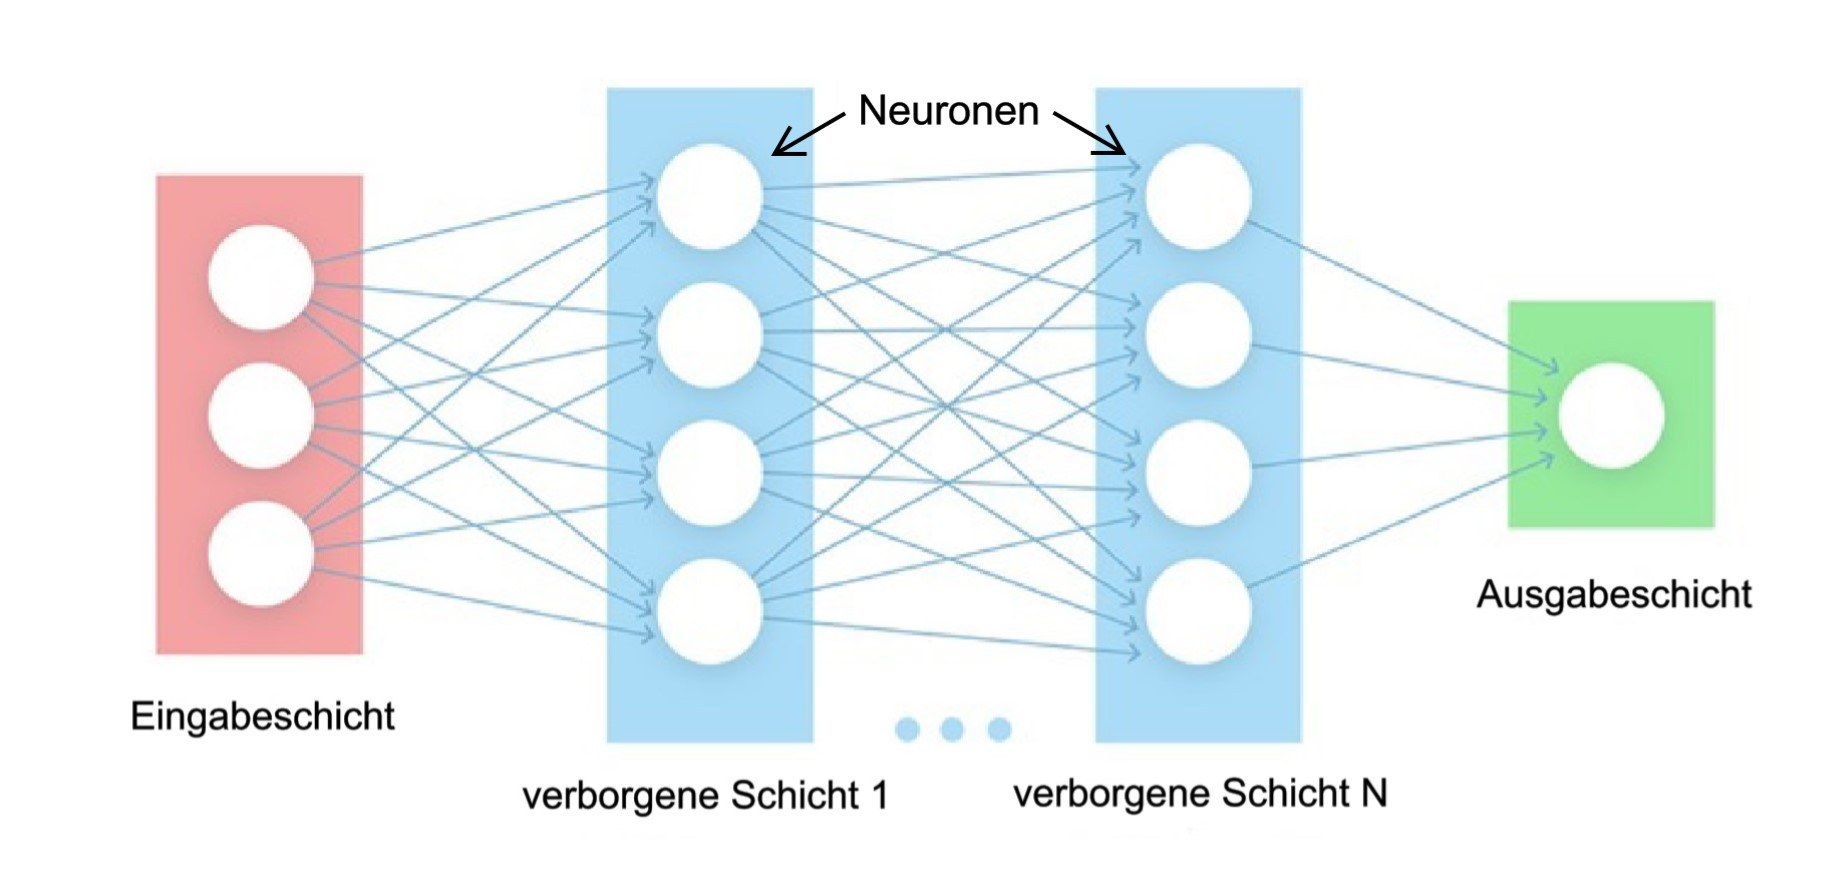
\includegraphics[width=\linewidth]{images/DNN}
	\caption{Aufbau eines (normalen) Deep Neural Networks \protect\cite{AufbauDNN}}
	\label{fig:DNN}
\end{figure}

\subsection{Backpropagation-Algorithmus}

DNNs lassen sich mittels des \emph{Backpropagation-Algorithmus} \cite{backpropapaper,Goodfellow-et-al-2016} trainieren. Der Algorithmus speist zunächst jede Trainingsinstanz in das zu trainierende DNN ein und berechnet die Ausgabe jedes Neurons in jeder konsekutiven Schicht (\emph{Forward Pass}). Danach ermittelt er den Ausgabefehler des DNNs (also die Differenz zwischen der gewünschten und der tatsächlichen Ausgabe), durchläuft jede Schicht in umgekehrter Richtung, um den Fehlerbeitrag jeder Neuronenverbindung auszurechnen (\emph{Backward Pass}). Basierend darauf optimiert der Backpropagation-Algorithmus die entsprechenden Verbindungsgewichte, um den Ausgabefehler des DNNs zu minimieren, was das Ziel des gesamten Trainingsprozesses ist.

Zur Steuerung des Trainingsprozesses im Backpropagation-Algorithmus kommen im Rahmen dieser Arbeit folgende Hyperparameter zum Einsatz.

\begin{description}
	\item[Batch-Größe] 
	
	Ein \emph{Batch} bezieht sich auf eine Menge von Trainingsbeispielen. Die Größe eines Batch ist die Anzahl der Trainingsinstanzen, die während eines Forward Pass in ein DNN eingespeist werden sollen, bevor die darin enthaltenen Verbindungsgewichte im darauffolgenden Backward Pass optimiert werden. Typischerweise wird die Batch-Größe je nach DNN-Modell auf 32 oder 64 gesetzt.
	
	\item[Lernrate] 
	
	Die Lernrate bezeichnet die Optimierungsrate der Gewichte eines DNN-Modells im Backpropagation-Algorithmus. Dieser Hyperparameter hängt eng zusammen mit \emph{Gradient Descent}, was ein Algorithmus innerhalb des Backpropagation-Algorithmus ist, der zur Optimierung der Verbindungsgewichte dient \cite{ruder2017overview,chandra2019gradient}. In der Praxis wird die Lernrate meistens auf $10^{-3}$ festgelegt.
	
	\item[Anzahl der Trainingsepochen]
	
	DNNs werden in der Regel mehrmals auf dem vorgegebenen Trainingsdatensatz trainiert. Dabei bezeichnet man jede Iteration als eine \emph{Trainingsepoche}. Während einer Epoche kann je nach Batch-Größe einer oder mehrere Batches trainiert werden.	
	 
\end{description}

\section{Convolutional Neural Network} \label{sec:cnn}

\subsection{Entwicklungsmeilensteine} \label{subsec:milestonecnn}

\begin{description}
	\item[1959 \& 1962]
		
	David H. Hubel und Torsten N. Wiesel untersuchten 1959 in \cite{PMID:14403678,PMID:14403679} und danach 1962 in \cite{PMID:14449617} durch eine Reihe von Experimenten an Katzen die Struktur vom \emph{visuellen Cortex}, der gemäß \cite{Bergua2017} die Region des Gehirns ist, die für die Verarbeitung und Integration der visuellen Information verantwortlich ist. Die Autoren entdeckten, dass viele Neuronen im visuellen Cortex ein kleines \emph{lokales rezeptives Feld} haben, d.~h. sie reagieren nur auf visuelle Stimuli, die sich in einem begrenzten Bereich des Gesichtsfeldes befinden (siehe \autoref{fig:1959CatExpr}, in der die lokalen rezeptiven Felder von fünf Neuronen durch gestrichelte Kreise dargestellt werden). Die rezeptiven Felder verschiedener Neuronen können sich überlappen und zusammen bilden sie das gesamte Gesichtsfeld. Außerdem fanden Hubel und Wiesel heraus, dass bestimmte Neuronen nur auf gewisse Arten von visuellen Stimuli reagieren, und dass einige Neuronen größere rezeptive Felder haben sowie auf komplexere Muster reagieren, die Kombinationen einfacherer Muster sind.
	
	\begin{figure}[!ht]
		\centering
		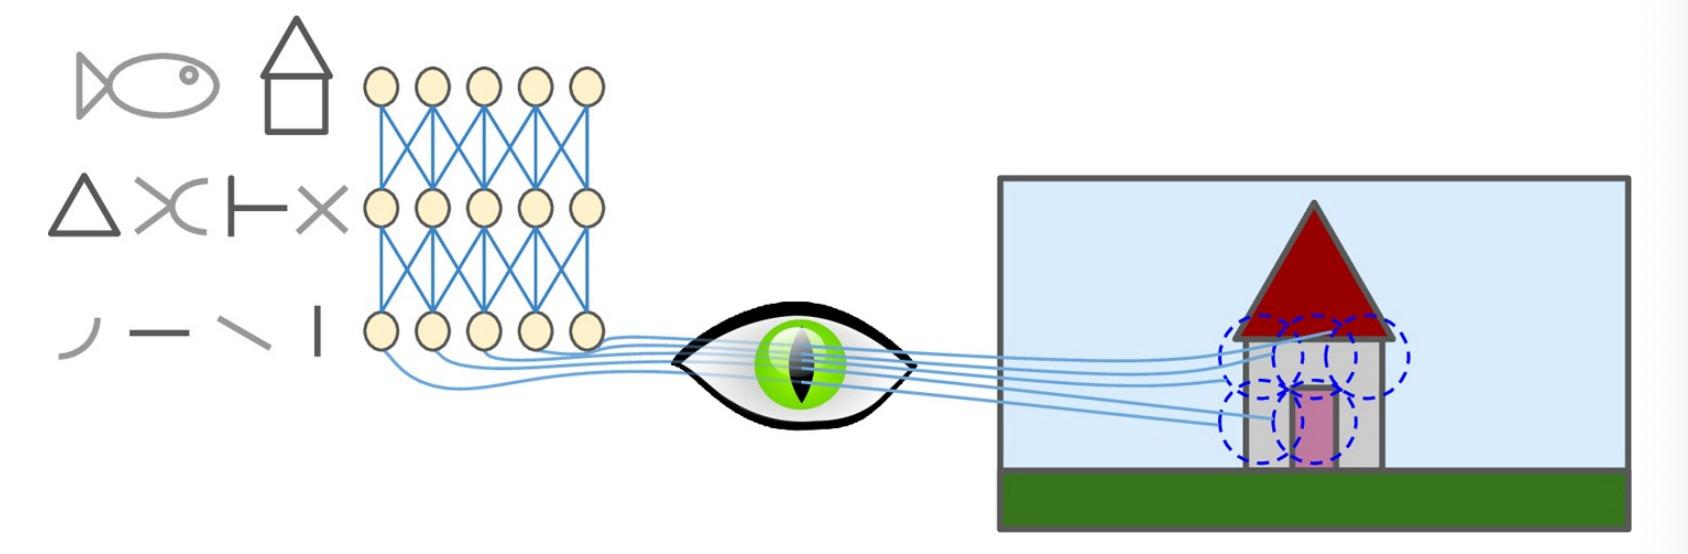
\includegraphics[width=\linewidth]{images/local_receptive_field}
		\caption{Lokales rezeptives Feld im visuellen Cortex \protect\cite{LocalReceptiveField}}
		\label{fig:1959CatExpr}
	\end{figure}
	
	Diese Beobachtungen führten zu der Idee, dass Neuronen eine hierarchische Organisation haben. Insbesondere basieren Neuronen höherer Schichten auf den Ausgaben benachbarter Neuronen in niedrigeren Schichten (Beachte in \autoref{fig:1959CatExpr}, dass jedes Neuron nur mit einigen wenigen Neuronen in der vorherigen Schicht verbunden ist). Diese Idee (im Weiteren als \emph{Hierarchical-Neural-Network-Idee} bezeichnet) schuf das erste wesentliche Fundament für die Entwicklung von CNNs.
		
	\item[1980 \& 1988] 
	
	Hubel und Wiesels Studien vom visuellen Cortex gaben Inspiration für das \emph{Neocognitron} von Kunihiko Fukushima, welches das erste Beispiel für eine Netzwerkarchitektur war, die die Hierarchical-Neural-Network-Idee in ihr Design aufnahm. Das Neocognitron ist ein 1980 in \cite{Neocognitron1980} vorgeschlagenes Modell für einen Mechanismus der verformungsbeständigen visuellen Mustererkennung. Später im Jahr 1988 wurde in \cite{Neocognitron1988} gezeigt, dass dieses Modell nach Training dazu in der Lage war.
	
	\begin{figure}[!ht]
		\centering
		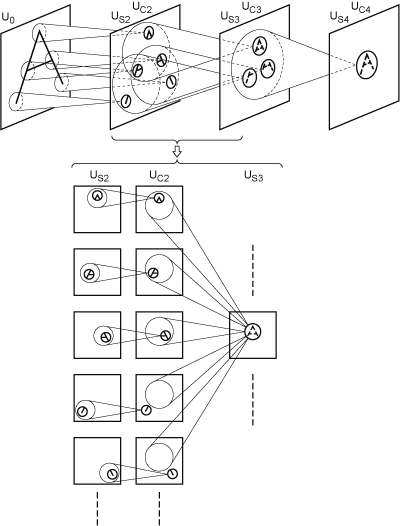
\includegraphics[width=0.72\linewidth]{images/Neocognitron}
		\caption{Der Prozess der Mustererkennung im Neocognitron. Die untere Hälfte der Abbildung ist eine vergrößerte Darstellung eines Teils vom Neocognitron. \protect\cite{neocognitron:scholarpediafig2}}
		\label{fig:neocognitron}
	\end{figure}

	Fukushima führte in seinem Neocognitron-Modell zwei besondere Komponenten ein: \emph{S-Zellen} und \emph{C-Zellen}. Der Einfachheit halber kann man Zellen als Neuronen betrachten. Während S-Zellen zur Merkmalsextraktion dienen, werden C-Zellen in das Neocognitron-Modell eingefügt, um Positionsfehler in den Merkmalen des Stimulus zu berücksichtigen. Die Zellen sind in abwechselnden Schichten von S-Zellen und C-Zellen angeordnet, sodass der Prozess der Merkmalsextraktion durch S-Zellen sowie der Tolerierung der Positionsverschiebung durch C-Zellen in der gesamten Netzwerkarchitektur wiederholt wird. Dadurch lassen sich lokale Merkmale, die in niedrigeren Schichten extrahiert wurden, schrittweise in globalere Merkmale integrieren (siehe \autoref{fig:neocognitron}). Die Schichten von S- sowie C-Zellen im Neocognitron sind jeweils die Vorläufer von den zwei grundlegenden Arten von Schichten in modernen CNN-Architekturen: \emph{Convolutional Layer} und \emph{Pooling Layer} (mehr dazu im \autoref{sec:CNN-Funktionale_Schichten}).
	
	\item[1989 \& 1998]
	
	Obwohl das Neocognitron-Modell 1980 erschien, wurde der Backpropagation-Algorithmus erst fast ein Jahrzehnt später in \cite{yannlecun1989} zum Trainieren von CNNs angewendet. Der Autor dieser Veröffentlichung, Yann LeCun, wandte erfolgreich eine Netzwerkarchitektur an, die eine Variante vom Neocognitron-Modell war und durch den Backpropagation-Algorithmus trainiert wurde, um handgeschriebene Postleitzahlen zu identifizieren. Diese Architektur ist die ursprüngliche Form von \emph{LeNet-5}, die als die bekannteste CNN-Architektur angesehen werden kann. LeNet-5 wurde erstmals 1998 in \cite{yannlecun1998} eingeführt. Dabei haben die Autoren verschiedene Methoden zur Erkennung von handschriftlichen Zeichen (einschließlich LeNet-5) überprüft und auf Basis ihrer Leistungen bei einer Standardaufgabe zur Erkennung handschriftlicher Ziffern verglichen. Die Ergebnisse zeigten, dass CNNs im Allgemeinen und LeNet-5 im Besonderen alle anderen Modelle übertrafen. Folglich war LeNet-5 in den folgenden Jahren der Ausgangspunkt für viele weitere CNN-Architekturen. Dieses Modell legte den Grundstein für das heutige Forschungsgebiet der Computer Vision.
	
	\item[2012]
	
	Jedoch war LeNet-5 aufgrund des Mangels an Rechenressourcen im Jahr 1998 noch nicht in der Lage, auf anspruchsvollere Daten als Ziffern zu skalieren. Um eine hohe Leistung bei komplexen Daten zu erzielen, war es notwendig, dass CNN-Modelle tiefer gehen und mehr Schichten haben, was für die damalige Zeit extrem rechenintensiv war. Dieses Problem ließ sich durch den Einsatz von Grafikprozessoren (GPUs) lösen. Diese Schlussfolgerung wurde 2012 von Alex Krizhevsky in \cite{10.1145/3065386} gezogen und durch sein CNN-Modell \emph{AlexNet} demonstriert. AlexNet ist größtenteils LeNet-5 ähnlich, nur viel größer und tiefer (in Bezug auf Größe und Anzahl der Schichten) und wurde mit zwei \emph{NVIDIA GeForce GTX 580} GPUs trainiert. Daneben war es die erste CNN-Architektur, die Convolutional Layers direkt übereinander legte, anstatt ein Pooling Layer über jedem Convolutional Layer zu platzieren (wie im Neocognitron-Modell von Fukushima). Mit großem Vorsprung hat diese Architektur den Wettbewerb ILSVRC 2012 gewonnen: Das Modell erreichte eine Top-5 Accuracy von 83\%, während das zweitbeste nur 74\% erreichen konnte\footfullcite{imagenet2012result}. Dies war das erste Mal, dass ein CNN-Modell auf dem großen ImageNet-Datensatz so gut funktionierte. AlexNet gilt somit als eine der einflussreichsten Veröffentlichungen im Bereich Computer Vision und hat viele weitere Forschungsarbeiten angeregt, die GPUs verwendeten, um das Training von CNNs zu beschleunigen.
	
\end{description}

\subsection{Unterschiede zwischen DNN- und CNN-Struktur}

CNNs sind ein Sondertyp von DNNs, der meistens für visuelle Anwendungen verwendet wird. Während die Leistung eines \emph{normalen DNNs} bei der Verarbeitung visueller Eingaben eingeschränkt ist, kann ein CNN dabei aufgrund von \emph{dreidimensionalen Neuronenblocks} und \emph{lokaler Konnektivität} eine hohe Leistung erreichen. 

Jede Schicht in einem normalen DNN lässt sich wie in \autoref{fig:3dcnn} links durch einen eindimensionalen Vektor darstellen. Außerdem ist jedes Neuron mit allen anderen Neuronen sowohl in der vorherigen als auch in der nächsten Schicht verbunden, daher werden die Schichten in einem normalen DNN auch als \emph{Fully-Connected Layer} bezeichnet. Allerdings ergeben sich zwei Probleme aus der \emph{eindimensionalen Darstellung von Schichten} sowie der \emph{vollen Konnektivität} in DNNs. Erstens, wenn die zwei- oder dreidimensionalen Bilder in eindimensionale Vektoren abgeflacht werden, können Zusammenhänge zwischen Pixeln, die zusammen ein Objekt im Bild bilden, verloren gehen. Zweitens lassen sich normale DNNs auf großformatige Bilder nicht gut skalieren, da die Anzahl der Gewichte, die zum Trainieren von normalen DNNs mit diesen Bildern benötigt werden, eminent hoch werden kann. Dies führt zu einem enormen Speicherbedarf des Computers, auf dem das Training durchgeführt werden soll.

\begin{figure}[!ht]
	\centering
	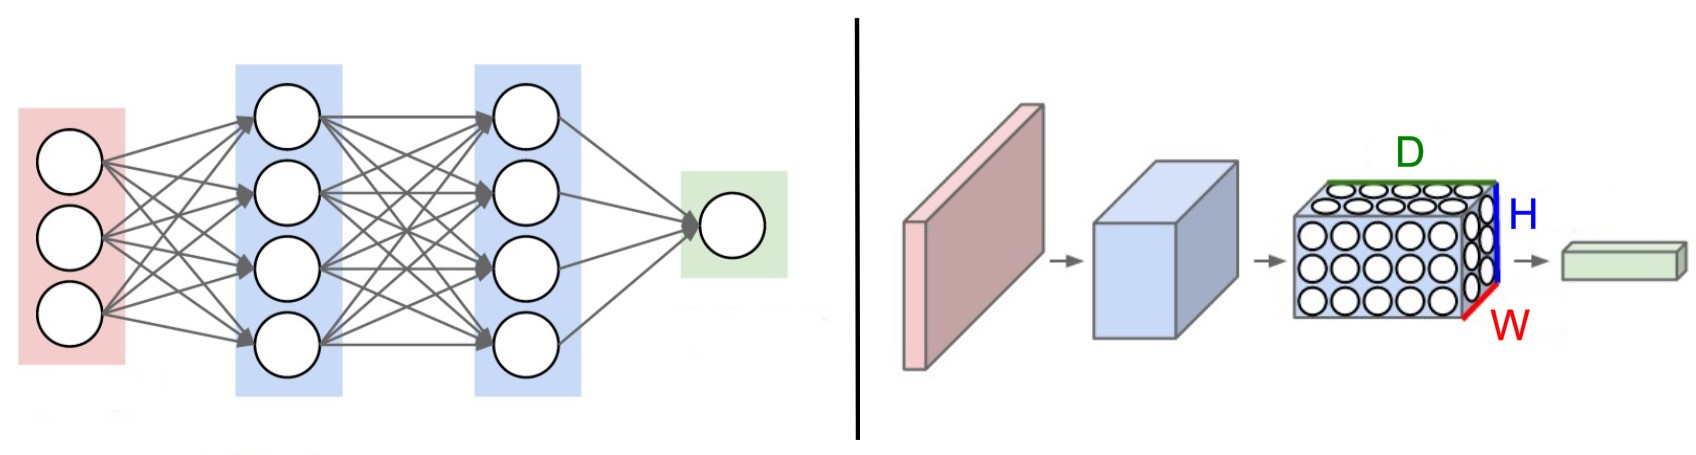
\includegraphics[width=\linewidth]{images/3DCNN}
	\caption{Links: Ein normales DNN. Rechts: Ein CNN, das die Neuronen jeder seiner Schichten in drei Dimensionen (Breite – W, Höhe – H, Tiefe – D) anordnet. Beachte, dass sich das Wort ''Tiefe'' hier auf die dritte Dimension eines Neuronenblocks bezieht, nicht auf die Gesamtzahl der Schichten in einem CNN.  \protect\cite{CS231nCNNarchitecture}}
	\label{fig:3dcnn}
\end{figure}

Ein CNN behandelt diese beiden Probleme, indem es dreidimensionale sowie teilweise verbundene Schichten in seiner Struktur verwendet:

\begin{description}
	\item[3D-Neuronenblocks]
	
	Wie der Name schon andeutet, wird jede Schicht eines CNNs wie in \autoref{fig:3dcnn} rechts als dreidimensionaler Neuronenblock dargestellt. Die drei Dimensionen der Eingabeschicht entsprechen jeweils der Höhe, Breite sowie Anzahl der Farbkanäle des Eingabebildes. Diese Darstellung sorgt dafür, dass die Zusammenhänge zwischen Pixeln im Eingabebild erhalten bleiben, was in normalen DNNs nicht möglich ist.

	\item[Lokale Konnektivität]
	
	CNNs sind so aufgebaut, dass jedes Neuron in einer Schicht nur mit einem kleinen Bereich der vorherigen Schicht (\emph{rezeptiven Feld}) verbunden ist, anstatt vollständig mit allen Neuronen davon. Diese Organisation kommt von der Hierarchical-Neural-Network-Idee von Hubel und Wiesel. Dadurch lässt sich die Anzahl der zu trainierenden Gewichte deutlich verringern, was die Skalierung von CNNs auf größere Bilder ermöglicht.
	
\end{description}

\subsection{Funktionale Schichten} \label{sec:CNN-Funktionale_Schichten}

Aus funktionaler Sicht bezieht sich eine CNN-Schicht auf eine Transformation und deren Ergebnis (siehe \autoref{fig:CNN_funktionale_schicht}). Im Allgemeinen sind sowohl die Eingaben als auch die Ausgaben jeder Transformation dreidimensionale Neuronenblocks, die als Stapel von \emph{Feature-Maps} betrachtet werden können. Bei einer Feature-Map handelt es sich um eine zweidimensionale Karte, die Merkmale kodiert, die durch Transformieren der Merkmale des Eingabeblocks erhalten werden. Je nach Art der Transformation unterscheidet man zwischen zwei Grundtypen von CNN-Schichten, nämlich Convolutional Layern und Pooling Layern.

\begin{figure}[!hb]
	\centering
	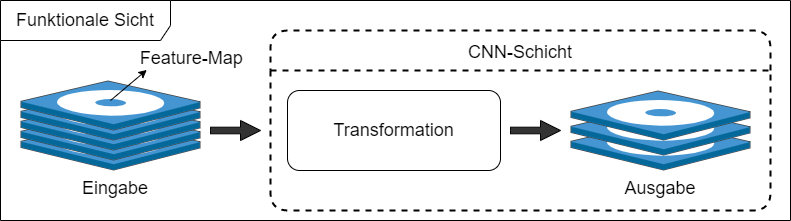
\includegraphics[width=\linewidth]{images/CNN_funktionale_schicht}
	\caption{CNN-Schicht aus funktionaler Sicht}
	\label{fig:CNN_funktionale_schicht}
\end{figure}

\begin{description}
	\item[Convolutional Layer] Wie die S-Zellen-Schichten im Neocognitron-Modell von Fukushima werden Convolutional Layer für die Merkmalsextraktion verwendet. Ein Convolutional Layer transformiert dazu Feature-Maps bzw. Merkmale im Eingabeblock in neue Maps mit komplexeren nützlicheren Merkmalen (siehe \autoref{fig:ConvLayerTransformationFilter}).
	
%\begin{figure}[!hb]
%	\centering
%	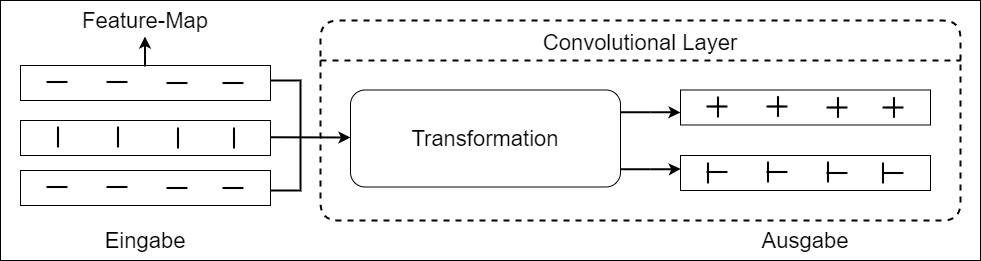
\includegraphics[width=\linewidth]{images/ConvLayerTransformation}
%	\caption{Transformation in Convolutional Layer}
%	\label{fig:ConvLayerTransformation}
%\end{figure}

	\begin{figure}[h]
		\centering
		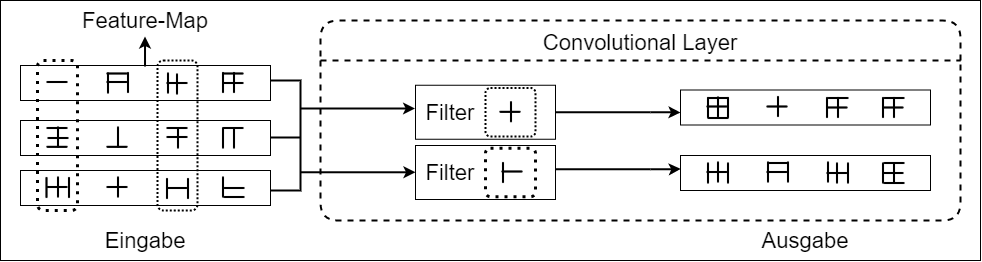
\includegraphics[width=\linewidth]{images/ConvLayerTransformationFilter}
		\caption{Convolutional Layer}
		\label{fig:ConvLayerTransformationFilter}
	\end{figure}
	
	Die Transformation in Convolutional Layern lässt sich durch sogenannte \emph{Filter} durchführen. Wie der Name verrät, werden während der Transformation mehrere Filter auf den ganzen Eingabeblock angewendet, und alle visuellen Merkmale darin, die den in diesen Filter angegebenen Merkmalen am ähnlichsten sind, werden extrahiert und in neue Feature-Maps integriert. In der Regel gilt, dass sich aus jedem Filter eine Feature-Map im Ausgabeblock ergibt. 
	
	Das Merkmal, das in einem Filter angegeben ist, wird ihm nicht manuell zugewiesen, sondern muss automatisch während des Trainingsvorgangs vom CNN gelernt werden. In der Tat ist ein Filter eine Zusammenstellung von Verbindungsgewichten, die mit dem Backpropagation-Algorithmus zu optimieren sind.
	%Während des Trainings findet ein CNN die nützlichsten Filter für seine Aufgabe und lernt, diese zu komplexeren Merkmalen zu kombinieren.
	\begin{figure}[!h]
	\centering
	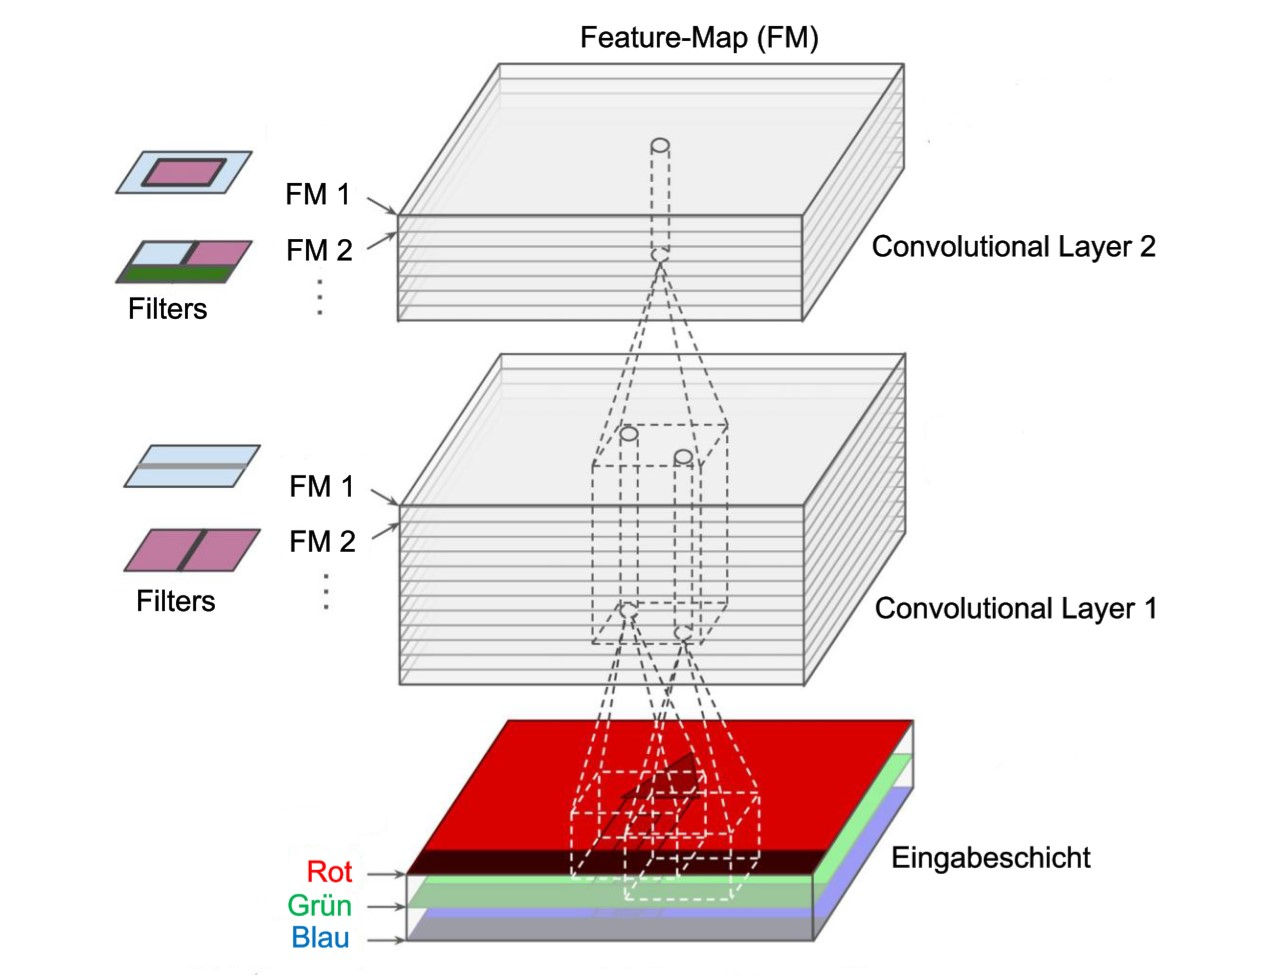
\includegraphics[width=0.95\linewidth]{images/convolutionalLayer}
	\caption{Merkmalsextraktion in Convolutional Layern  \protect\cite{convlayer}}
	\label{fig:convlayer}
	\end{figure}

	\autoref{fig:convlayer} bildet die Merkmalsextraktion in Convolutional Layer in funktionaler sowie struktureller Hinsicht ab. Zur Merkmalsextraktion läuft ein Filter über die gegebene Schicht und verarbeitet sukzessiv alle lokalen rezeptiven Felder darin (gestrichelte Quader in der Abbildung). Die Gewichte eines Filters sind für alle rezeptiven Felder dieselben. Das Ergebnis der Verarbeitung eines Felds ist ein Wert, der einem Neuron zugeordnet wird (lokale Konnektivität), und zusammen bilden alle Neuronen, die aus demselben Filter resultieren, eine Feature-Map in einem Convolutional Layer. Detailliertere Informationen dazu befinden sich in \cite{10.5555/3378999}.

	\item[Pooling Layer] Pooling Layer dienen nicht nur zur Tolerierung der Positionsverschiebung wie die C-Zellen-Schichten im Neocognitron-Modell, sondern auch zur Reduzierung der Rechenlast, Speichernutzung und Anzahl der Verbindungsgewichte. Diese Ziele lassen sich durch Unterabtasten (Schrumpfen) des Eingabeblocks erreichen. In anderen Worten transformiert ein Pooling Layer Feature-Maps im Eingabeblock in kleinere Feature-Maps aber mit den gleichen Merkmalen (siehe \autoref{fig:PoolingLayerTransformationFilter}).
	
	%\begin{figure}[!hb]
	%	\centering
	%	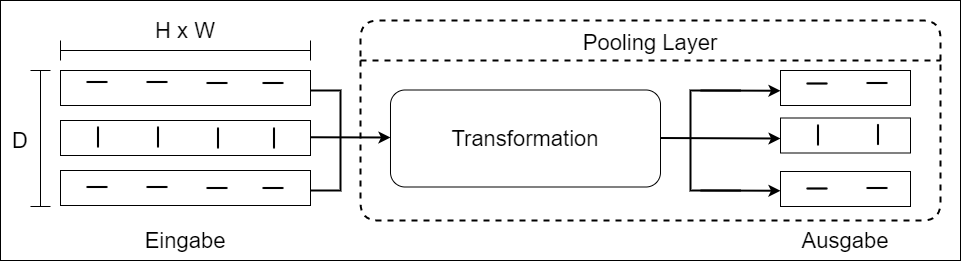
\includegraphics[width=\linewidth]{images/PoolingLayerTransformation}
	%	\caption{Transformation in Pooling Layer}
	%	\label{fig:PoolingLayerTransformation}
	%\end{figure}

	\begin{figure}[!h]
		\centering
		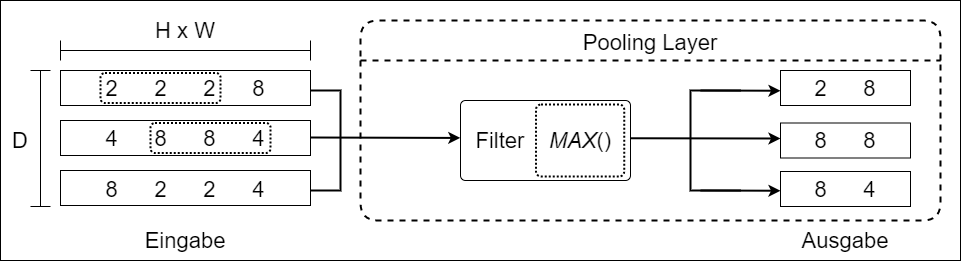
\includegraphics[width=\linewidth]{images/PoolingLayerTransformationFilter}
		\caption{Pooling Layer}
		\label{fig:PoolingLayerTransformationFilter}
	\end{figure}

	Die Transformation in Pooling Layern lässt sich auch durch Filter durchführen. Es gilt ebenfalls die Regel, dass sich aus jedem Filter eine Feature-Map im Ausgabeblock ergibt. Trotzdem haben diese Filter im Gegensatz zu denjenigen in Convolutional Layern keine Verbindungsgewichte, d.~h. sie werden nicht trainiert, sondern wenden lediglich eine der Aggregatfunktionen auf die Feature-Maps an, um Merkmale darin zu aggregieren und dadurch die Größe der Feature-Maps zu verkleinern. Beispielsweise wird in \autoref{fig:PoolingLayerTransformationFilter} ein Filter der Art $MAX()$ zunächst auf die ersten drei Merkmale jeder Feature-Map angewendet und anschließend auf die letzten drei (Jede Zahl entspricht einem Merkmal). Die resultierenden Feature-Maps sind dank der Aggregation nur halb so groß wie zuvor.

\end{description}

Typischerweise werden Convolutional und Pooling Layers zusammen mit Fully-Connected Layern kombiniert und in einer bestimmten Reihenfolge angeordnet, um ein CNN-Modell z.~B. zur Bildklassifizierung aufzubauen (siehe \autoref{fig:imgKlassifizierungProzess}). Wenn das Eingabebild die Schichten in einem solchen CNN-Modell durchläuft, wird es immer kleiner, aber durch die Anwendung einer steigenden Anzahl Filter pro Convolutional Layer immer tiefer (d.~h. dieses Bild hat mehr Feature-Maps). In diesem Modell enthält die Eingabeschicht die rohen Pixelwerte vom Eingabebild, während die Ausgabeschicht mittels \emph{Softmax-Funktion}\footfullcite{Softmax} einen eindimensionalen Vektor der Größe $K$ (Anzahl der Klassen) ausgibt, wobei jeder Komponentenwert einer Wahrscheinlichkeit entspricht, dass das Eingabebild zu einer bestimmten Klasse gehört.

\begin{figure}[!h]
	\centering
	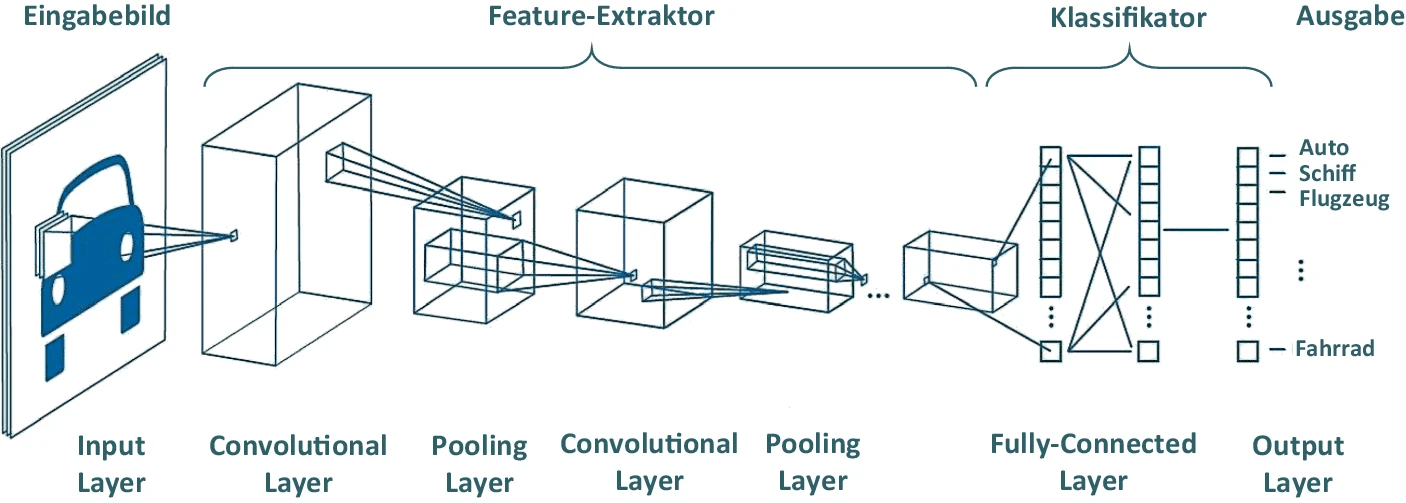
\includegraphics[width=\linewidth]{images/imgKlassifizierungProzess}
	\caption{Allgemeiner Aufbau eines CNNs \protect\cite{Zschech2021}}
	\label{fig:imgKlassifizierungProzess}
\end{figure}
